\section{Energy Consumption}
This section presents the definition of energy, what are the relevant hardware components on energy consumption, which methods exist to measure energy consumption, and more detailed insight into the tools used in this work.

\subsection{Energy and Power} \label{energypower} 
In order to understand how energy consumption can be measured, we must first understand what power is, what energy is and how different it is.

The scientific definition of Power is the total workload or energy transferred divided by the time interval. In this context, power is the amount of energy consumed per unit of time. According to The international system of units~\cite{taylor_1991}, the universal unit used for power is Watts (W) or Joules/s. Energy is the total workload of a system during a period of time and is the unit used for Energy is Joules (J).

The Power can be calculated in two ways, the first is when we know the total energy and the time interval,

\begin{equation}
P = \frac{E}{\Delta t} 
\end{equation}

The other possible way of calculating is through Voltage and current intensity. Voltage is defined to be the potential energy of two different points and the Unit is Volts and Current intensity is the magnitude of an electric current as measured by the quantity of electricity crossing a specified area of equipotential surface per unit time and unit of measurement is Amperes (A). 

With this we can calculate the power by this formula:

\begin{equation}\label{eq:pvi}
P = V I
\end{equation}

With this two formulas we can deduce this formula to calculate the energy,

\begin{equation}\label{eq:energyfinal}
E = V I \Delta t
\end{equation}

\begin{table}[H]
\centering
\begin{tabular}{l|c|c|}
\cline{2-3}
                              & Unit        & Symbol \\ \hline
\multicolumn{1}{|l|}{Voltage} & Volt (V)    & V      \\
\multicolumn{1}{|l|}{Current} & Amperes (A) & I      \\
\multicolumn{1}{|l|}{Energy}  & Joules (J)  & E      \\
\multicolumn{1}{|l|}{Power}   & Watts (W)   & P      \\ \hline
\end{tabular}
\caption{List of electrical properties, units, and symbols}
\end{table}

The formulas below gonna be important because without them we can't measure energy by a direct approach.

\subsection{Types of Energy Consumption}
To measure the total and individual components energy consumption, first we have to divide the energy consumption in different groups. There are several ways to group a device's overall energy consumption by measuring the level of use of hardware resources in the system. This analysis can be separate the energy consumption of a system into two categories: static energy consumption and dynamic energy consumption.

\begin{itemize}
    \item \textbf{Static Consumption:} is the base consumption needed to ensure that the system is ready, and able to respond to any user need quickly and effectively. This energy is consumed by the system regardless of the state of operation. This includes energy consumed inactive by the disks, network interfaces, \gls{cpu}, caches, memory, motherboard, etc. This category also includes the energy needed to maintain the basic requirements of the operating system and other tasks in progress~\cite{portela2016}.
    
   \item \textbf{Dynamic Consumption:} This refers to the basic consumption necessary for an operation requested by the user of the system. Dynamic Energy includes the energy consumed by the \gls{cpu}, the extraordinary operations on the \gls{dram}, the disk when searching, reading or/and writing data, the network interface when receiving and transmitting data packets, and other needs to respond to user requests when executing instructions. Dynamic power consumption values mainly depend on the type of workload that runs on the machine. ~\cite{portela2016}.
  \end{itemize}
  

\subsection{Relevant Hardware Components}

Before we design a model of energy consumption, first we need to understand which hardware components are relevant to global consumption. This is a relevant point because while static consumption has an unchanging base value and is easy to capture, dynamic consumption varies constantly and sometimes it becomes difficult to find any coherence in that variation. 

According to several studies carried out during the last 15 years, it shows that the main subsystems that generate dynamic energy consumption are the CPU, the Memory, and Disk~\cite{portela2016}. According to google research \cite{google} provided some insight into how energy is used in modern IT equipment at the time and got by breaking down the peak power usage of one generation of WSCs deployed at Google in 2007 categorized by main component group, they got that using modern data center using late 2012 generation servers the 3 main hardware components besides cooling components on energy total consumption was \gls{cpu} with 42\%, Disks with 14,3\% and \gls{dram} with 12,3\%. Also \citeauthor{kensal} mentions in an article that the subsystems with more impact on the dynamic consumption are CPU, memory and disk, represent, respectively, 58\%, 28\% and 14\% .

With this information, we can conclude that our energy model must be around this 3 components and it also facilitates the study of the causes of energy variations in the DBMS. 
%Google, L. A. Barroso e U. Hölzle, The Datacenter as a Computer: AnIntroduction to the Design of Warehouse-Scale Machines, vol. 6,Morgan & Claypool Publishers, 2009. 


\subsection{Methods To Measure Energy Consumption}


With the unit of measure energy determined in section \ref{energypower}, in this subsection it will be explain the three ways that energy can be measure. This methods are \cite{ardito2019methodological}:

\begin{itemize}
    \item \textbf{Instant Power Measurement:} The instantaneous current consumed by the unit is determined by his technique and then multiplied by the voltage. The integral gives the energy value over a period. If the sampling frequency is high, instant power measurements are reliable, but they require physical instrumentation. This method generally works at the level of the system, although measuring the component-level of hardware is possible.
    \item \textbf{Time Measurement:} Another way to collect the energy consumption of a device is through measurement of time. Assuming a constant consumption over time, the speed at which energy is depleted depends on the power consumption of the device. 
    \item \textbf{Model Estimation:} Energy consumption calculations in this method are measured in a way where a power consumption of a specific computer is connected to internal resource use indicators, such as \gls{cpu} states, commands, memory or disk access, and network adapters. This method utilizes machine calls to estimate the usage of resources.
\end{itemize}

\subsection{Energy Measurement Tools}
In this subsection, it is shown which Energy measurement tools are used in this study and a quick understanding of how they work.

\subsubsection{RAPL}
   Intel’s \gls{rapl} is a tool to measure the energy on \gls{cpu} and primary storage (\gls{dram}). Here it will explain how it got introduce, how it works, and the limitations it has.
	
	\gls{rapl} is a well-known and accepted interface for measuring the power consumption of a computer system. Various studies used this interface as a measuring tool, and others review Intel \gls{rapl} measurements in terms of accuracy, performance, granularity, usability ~\cite{raplpref,raplpref2}.
	

	Intel introduced \gls{rapl} on they compilers in the architecture of the Intel Sandy Bridge, and since the first appearance, it has been evolving in the newer architectures. \gls{rapl} has \gls{msr} that aren't part of the architecture of the processor but address power values required for energy consumption management ~\cite{raplpref,intel64and,portela2016}.
	
	
    The mains functionalities of the \gls{rapl} are to measuring the energy consumption on the \gls{cpu} and primary storage and also to limit the energy consumption on the components mentions. In the context of this research, we won't use the last functionality, as it does not fit in the context of this study ~\cite{raplpref,raplpref2,intel64and}.
	
	
	The \gls{rapl} does not measurements energy based on an analog energy meter because energy consumption is estimated through the analysis of various hardware performance counters, temperature sensors, leakage energy, and IO models.  Registers reserved for energy readings are updated approximately every millisecond (1kHz) ~\cite{energypapi,portela2016}.

    \begin{figure}[ht!]
    \centering
    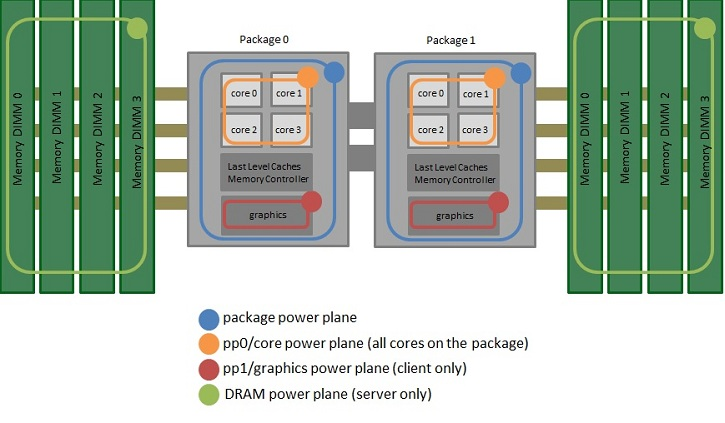
\includegraphics[width=\linewidth]{Chapters/images/power_domains2.jpg}  \caption{Intel’s \gls{rapl} Power Domain.}
    \label{fig:powerdomain}
    \end{figure}
    
    We can check the different power domains supported by \gls{rapl} in figure \ref{fig:powerdomain}. Each power domain has a different  \gls{msr}  and reports the domain's energy consumption, allowing us to limit that domain's power usage over a specified time. Each domain represents distinct physical component sets, currently, these are: 
    
    \begin{itemize}
        \item \textbf{Package}: the package domain refers to the package's energy consumption of the entire socket, including the core and uncore components energy ~\cite{intel64and}.
        \item \textbf{PP0/Core Power Plane 0}: This domain measurement the energy consumption of all processors socket~\cite{intel64and,portela2016}.
            \item \textbf{PP1/Graphics Power Plane 1}: This domain measures the energy consumed by all processors in a \gls{gpu}.
        \item \textbf{DRAM}: This Domain refers to the energy consumption of random access memory (RAM)~\cite{intel64and,portela2016}.
        \item \textbf{Psys}: Intel \textit{Skylake} has introduced a new \gls{rapl} Domain named PSys. It monitors and controls the thermal and power specifications of the entire SoC and it is particularly useful when the source of power consumption is neither the \gls{cpu} nor the \gls{gpu} \cite{raplpref}.
    \end{itemize}
    For multi-socket server systems, each socket reports its own \gls{rapl} values \cite{raplpref}.
    
    There are some distinctions between the list of available domains, depending on the type of platform. The available domains on platforms intended for the client are Package, Power Plane (PP) 0, and PP1. On the other hand, the Package, PP0, and \gls{dram} domains are available on the Platform intended for Servers \cite{raplpref2}.
    In the Table \ref{tab:rapltable} presents an overview of \gls{rapl} domains supported by different processor model.
% Please add the following required packages to your document preamble:
% \usepackage{multirow}
\begin{table}[H]
\centering
\caption{RAPL power domains supported by different models}
\begin{tabular}{|c|c|c|c|c|c|}
\hline
\multirow{ }{Model }{} & \multicolumn{5}{c|}{Power domain supported} \\ \cline{2-6} 
                       & PKG    & PPO    & PP1    & DRAM    & PSYs   \\ \hline
Sandy Bridge           & YES    & YES    & YES    & NO      & NO     \\
Sandy Bridge-EP        & YES    & YES    & NO     & YES     & NO     \\
Haswell                & YES    & YES    & YES    & YES     & NO     \\
Haswell-EP             & YES    & NO     & NO     & YES     & NO     \\
Skylake                & YES    & YES    & YES    & YES     & YES*   \\ \hline
\end{tabular}
\label{tab:rapltable}
\newline
*Not All Skylake versions support PSys

\end{table}

    The MSR interfaces available in each of the domains mentioned are the following:
\begin{itemize}

    \item \textbf{Power Limit}: interface serves to specify the time interval and the limit of energy to be consumed~\cite{raplpref2,portela2016}. 
\item \textbf{Energy Status}: This interface provides the energy consumed. The register reports the actual power used by the domain. This interface is read-only. 
\item\textbf{Perf Status}: This interface is optional and provides the effects of restrictions used~\cite{intel64and,portela2016}.
\item \textbf{Power Info}: This interface is optional and presents the information for a given domain (Power, Energy, etc.)~\cite{portela2016}.
\item \textbf{Policy}: This Interface is optional and it allows defining control policies for energy to distribute costs, that is, to balance the power consumed between domains subdomains ~\cite{raplpref2}. 
\end{itemize}

With all this information we can conclude that the largest domain we can get on \gls{rapl} is with this equation:

\begin{equation}
E_{PPO} + E_{PP1} <= E_{Packgage}
\end{equation}$
$

To gather results, we develop software in C, that is running in parallel with the task we want to measure. On the listing \ref{lst:raplcode} , is a example of the code we made.

    
    \begin{lstlisting}[ caption={ Exemple of reading RAPL energy in C},label={lst:raplcode},language=C,
    basicstyle=\tiny, %or \small or \footnotesize etc.
]
void rapl_after(FILE * fp , int core){ 
  int fd;
  long long result;
  fd=open_msr(core);

  result=read_msr(fd,MSR_PKG_ENERGY_STATUS);
  package_after=(double)result*energy_units;
  fprintf(fp,"%.6f , ",package_after-package_before);  // PACKAGE

  result=read_msr(fd,MSR_PP0_ENERGY_STATUS);
  pp0_after=(double)result*energy_units;
  
  fprintf(fp,"%.6f , ",pp0_after-pp0_before);    // CORE

  if ((cpu_model==CPU_SANDYBRIDGE) || (cpu_model==CPU_IVYBRIDGE) ||
	(cpu_model==CPU_HASWELL)) {
     result=read_msr(fd,MSR_PP1_ENERGY_STATUS);
     pp1_after=(double)result*energy_units;
     fprintf(fp,"%.6f , ",pp1_after-pp1_before);     // GPU
  }
  else fprintf(fp,"  , ");   
  
  if ((cpu_model==CPU_SANDYBRIDGE_EP) || (cpu_model==CPU_IVYBRIDGE_EP) ||
	(cpu_model==CPU_HASWELL)) {
     result=read_msr(fd,MSR_DRAM_ENERGY_STATUS);
     dram_after=(double)result*energy_units;
     fprintf(fp,"%.6f , ",dram_after-dram_before);     // DRAM
  }
  else fprintf(fp,"  , "); }
\end{lstlisting}


    The \gls{msr} driver must be enabled for direct MSR access with \textit{/dev/cpu/*/msr} command, and read access permission must be set for the driver. Reading \gls{rapl} domain values directly from \gls{msr} requires the \gls{cpu} model to be detected and the \gls{rapl} energy units read before reading the consumption values of the \gls{rapl} domains ~\cite{raplpref,energypapi}. Once the \gls{cpu} model is detected, the \gls{rapl} domains can be read per package of the \gls{cpu} by reading the corresponding “MSR status” register  ~\cite{raplpref,intel64and}.

\subsubsection{Arduino}
To benchmark the energy consumption on disk storage, we had to choose between indirect methods or direct methods.

%The Indirect methods consist of estimating the energy base how much time he spent in which state and how much the seeks, reads, and writes, and knowing much which operation costs and how much energy he spent every time he which is every state. With that knowledge, we can estimate how much energy consumption during that time. This approach produces good results, but since all energy is an estimate, this procedure including an error margin on the results.

%The other approach is the direct method by using external hardware, this method consists of measuring Electric Potential Difference on the disk. This method is a lot precise since the results are real, but the downsize it is that have an impact on the overall performance, this impact it only notices on a big scale~\cite{portela2016}.

It was opt-in for a instant power measurement approach because this was the simplest and sufficient solution to achieve the objectives intended of reading, constantly and automatically the energy consumption on the secondary storage ensuring that our results are precise and reliable and since our measurements are on a small scale it doesn't have an impact on the overall systemy~\cite{portela2016}.

Since it is necessary data handling on our behalf and because we need to store energy spent, a normal ammeter won't do the work. Thus to gather our measurements we choose to use an Arduino Uno with a current sensory~\cite{portela2016}.

The SATA cable is responsible for distributing energy to the disk and data exchange between the secondary memory and the computer. So to get the energy on the disk we must connect the current sensor to the connection of the SATA cable that is responsible for distributing energy~\cite{portela2016}.

The current sensor we opt-in was the Low Current Sensor Breakout. This current sensor is marketed by SparkFun and can measure the current regardless of whether the signal is continuous or alternating. The sensor is also accompanied by an operational amplifier phase to control the gain, which can measure lower currents more precisely ~\cite{portela2016}.

\begin{figure}[H]
  \caption{Scheme of connections between Sata cable, current sensor and Arduino used to measurement secondary storage.}
  \centering
  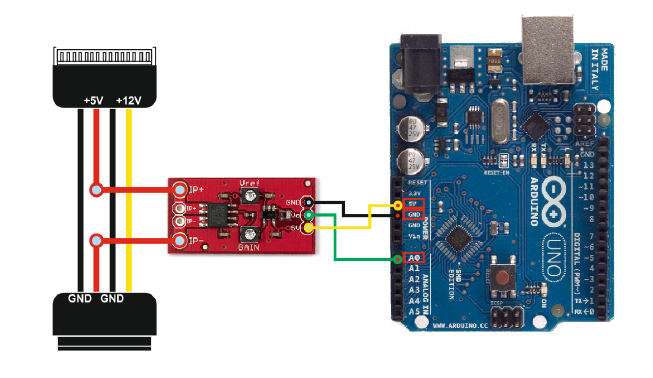
\includegraphics[width=\linewidth]{Chapters/images/arduino.png}
\end{figure}

Also, an Arduino UNO was used to read the analog voltage presented by the sensor and communicate these values to the computer connected to it through the serial port. For this, we had to develop a program for the Arduino that would get take constant readings at the analog voltage and send them every 0.1 seconds. 

  \begin{lstlisting}[ caption={ Arduino source code for reading the analog signal from the current sensor},label={lst:arduinocode},language=C,
    basicstyle=\small
]
void loop() {
  /* Initialization */
  float average_a0 = 0; // Raw reading from pin
  float voltage = 0; // Voltage in V
  float current = 0; // Current in A
  float wattage = 0; // Wattage in W
  float power = 0; // Power in J
  /* Average loop */
  for(int i = 0; i < n_reads ; i++) {
    average_a0 += analogRead(sensorPin_0);
    delay(loop_delay);  }
  /* Formula based computations */
  average_a0 /= n_reads;
  voltage = (average_a0 / 1024.0) * 5;
  current = current_eq(voltage);
  wattage = voltage * current;
  power = wattage * interval;
  Serial.println(power, 3);
  Serial.flush();}

\end{lstlisting}


Following the code on the listing \ref{lst:arduinocode}, the reading is made every millisecond and then is made the average of the last one hundred milliseconds, which is finally sent to the computer system connected to the Arduino.

